\section{Pemrosesan \textit{Stream}}

Secara umum, \textit{stream} merujuk pada data yang tersedia secara inkremental dari waktu ke waktu. Konsep ini dipakai di berbagai tempat, seperti stdin dan stdout Unix, koneksi TCP, dan lain-lain \parencite{dataIntensiveApplications}.

\textit{Stream processing} merupakan paradigma pemrograman yang memandang \textit{stream} atau urutan \textit{event} sebagai objek masukan dan luaran utama dari komputasi. \cite{streaming101} menyatakan bahwa \textit{stream processing} merupakan tipe mersin pemrosesan data yang didesain dengan mempertimbangkan data yang tidak terbatas.

\cite{streamProcessingComparison} menyatakan bahwa terdapat karakteristik penting pada \textit{stream processing}, yaitu:

\begin{enumerate}
    \item \textit{Delivery guarantees}. Setiap informasi yang masuk harus dijamin akan diproses oleh \textit{streaming engine}.
    \item Toleransi kegagalan (\textit{fault tolerance}). Ketika terjadi kegagalan, \textit{streaming engine} harus mampu melakukan pemulihan dan memulai ulang dari titik yang ditinggalkan.
    \item \textit{State management}. \textit{Streaming engine} harus memiliki mekanisme untuk menyimpan dan memperbarui informasi \textit{state}.
    \item Memiliki kinerja yang baik dari sisi latensi, \textit{throughput}, dan skalabilitas.
    \item Memiliki fitur yang lebih canggih, seperti \textit{event time processing}, \textit{watermarks}, \textit{windowing}, dan lain-lain.
\end{enumerate}

Selain itu, karakteristik \textit{stream processing} juga bisa dibagi menjadi dua jenis, yaitu:

\begin{enumerate}
    \item \textit{Native streaming}. \textit{Stream processing} jenis ini akan langsung memproses data yang diterima secepat mungkin. Contoh \textit{stream processing} tipe ini adalah Apache Storm, Apache Flink, Apache Kafka Streams, dan Apache Samza.
    \item \textit{Micro-batching}. \textit{Stream processing} jenis ini memproses data setiap beberapa detik atau milidetik sekali sehingga data diproses dalam setiap kelompok kecil dengan sedikit keterlambatan. Contoh \textit{stream processing} tipe ini adalah Apache Spark Streaming dan Apache Storm-Trident.
\end{enumerate}

\subsection{RisingWave}

RisingWave merupakan \textit{cloud-native streaming database}. Setelah menghubungkan sumber \textit{stream}, pengguna dapat membuat kueri analisis dengan mendefinisikan \textit{materialized view}, yang diperbarui secara inkremental pada RisingWave \textit{streaming engine} \parencite{risingwave}.

Berikut adalah keuntungan RisingWave:

\begin{enumerate}
    \item Mudah dipelajari karena merupakan ekstensi dari sintaks PostgreSQL.
    \item Mudah dioperasikan dan memiliki kebutuhan sumber daya yang lebih rendah karena ditulis dalam bahasa sistem Rust.
    \item Mendukung berbagai sumber data dan mampu mengirimkan (\textit{sink}) data ke dalam berbagai sumber, seperti mengambil data dari Apache Kafka lalu hasilnya dikirim ke ClickHouse. RisingWave mendukung integrasi dengan PostgreSQL CDC dan Apache Kafka sebagai sumber (\textit{source}) dan tujuan data (\textit{sink}).
    \item Menjamin konsistensi pada \textit{materialized view} dengan menggunakan \textit{snapshot}.
\end{enumerate}

\begin{figure}[ht]
    \centering
    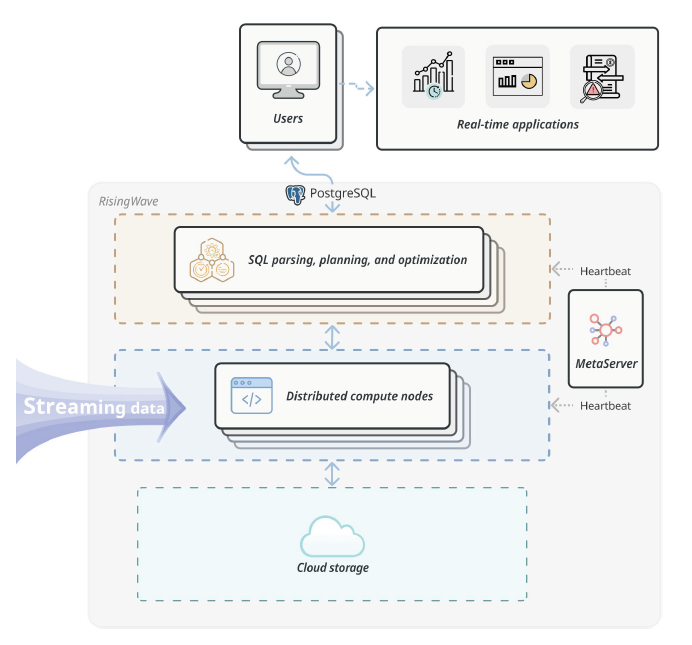
\includegraphics[width=0.8\textwidth]{resources/chapter-2/risingwave.png}
    \caption{Arsitektur RisingWave \parencite{risingwave}}
    \label{fig:risingwave-architecture}
\end{figure}

Node komputasi pada RisingWave terdiri atas \textit{batch engine} dan \textit{streaming engine}. \textit{Batch engine} meliputi \textit{query execution engine} dan \textit{exchange service} untuk menukar data antar node komputasi. \textit{Streaming engine} dibangun atas model aktor pada pemrograman konkuren. Mesin ini berinteraksi langsung dengan \textit{frontend} dan melayani \textit{stream data}. Selain itu, terdapat \textit{meta service} yang berperan sebagai layanan sentral untuk menyimpan metadata seperti keadaan kluster, katalog sistem, keanggotaan kluster, dan lain-lain \parencite{risingwave}.